\chapter{The service}\label{the-service}

\section{What is Neosluger?}\label{what-is-neosluger}

Neosluger\footnote{
	\url{https://github.com/OSL-UGR/neosluger}
} is a complete rewrite of the University of Granada's URL shortener Sluger\footnote{
	\url{https://github.com/OSL-UGR/sluger}
},
which stands for \textbf{S}hort \textbf{L}ink \textbf{UGR} (and \textit{e} is added as a pronunciation aid).
It is Free Software, which means that you are free to modify and distribute it as long as you do so bounded by the limits and obligations of its licence.

The old version offered a URL shortener, an API and public access stats for each short link.
This version renews the API and offers a QR code generator that can be freely used for any link, not only the officially shortened ones.
As with the old version, the URL shortener is only available for users accessing the service from the University of Granada's network, but all other services are available to the general public.
This is done to ensure that all links are created for purposes related to the University.

The new service is available in the same address as the original one: \url{https://sl.ugr.es/}

\section{The web interface}\label{the-web-interface}

\begin{figure}[ht!]
	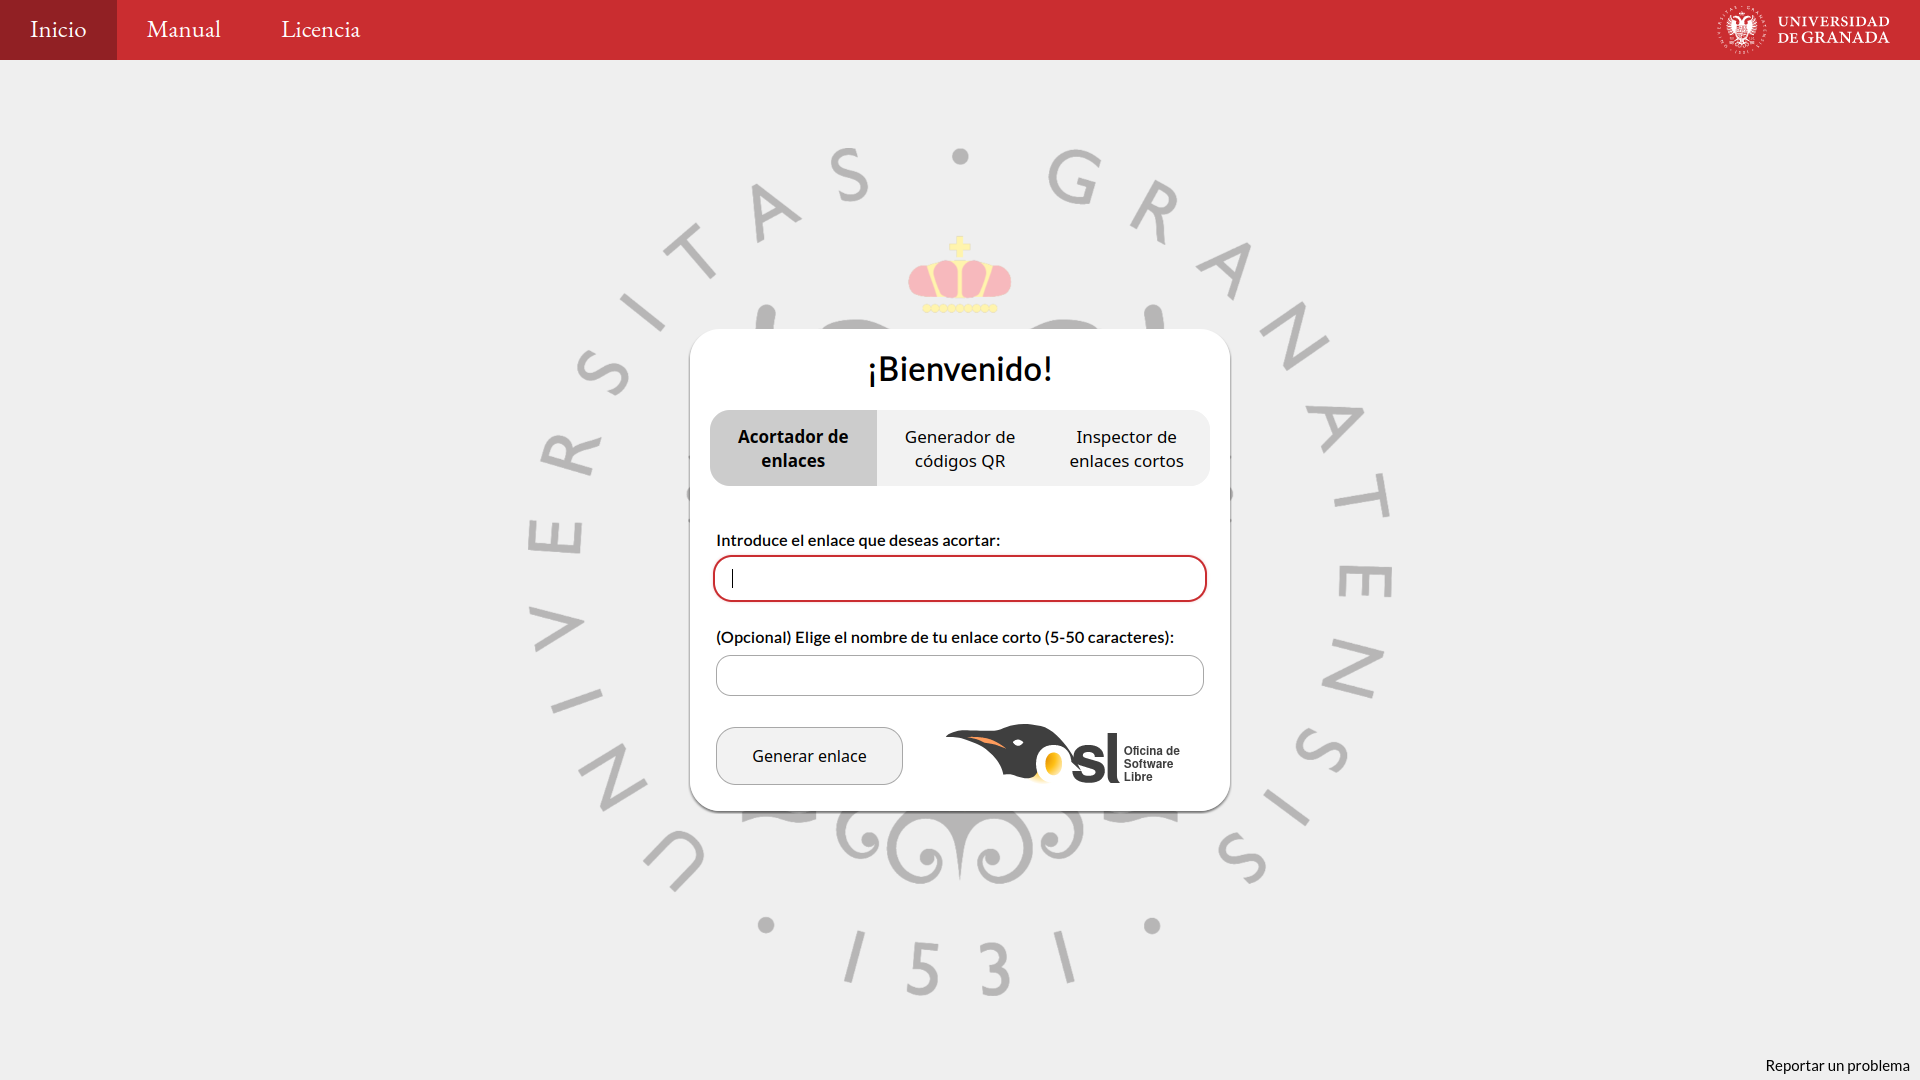
\includegraphics{web-index}
	\caption{Neosluger's index page.}
\end{figure}

Neosluger's web interface consists of three tabs:
The index tab (\textit{Inicio}) is the one the user sees first and contains the URL shortener (\textit{Acortador de enlaces}), the QR code generator (\textit{Generador de códigos QR}) and the shortened URLs inspector (\textit{Inspector de enlaces cortos}).

The manual page contains instructions for the URL shortener (\textit{Acortador de enlaces}), the QR code generator (\textit{Generador de códigos QR}) and the API.
The licence page contains the service's licence, a link to the original text by GNU, a raw version of the licence and a link to Neosluger's repository.
Every pages contains a report button (\textit{Reportar un problema}) that guides the user to a report page where they can get in contact with the University's Office for Free Software to change or delete a link or to have a feature fixed as soon as possible.

\begin{figure}[ht!]
	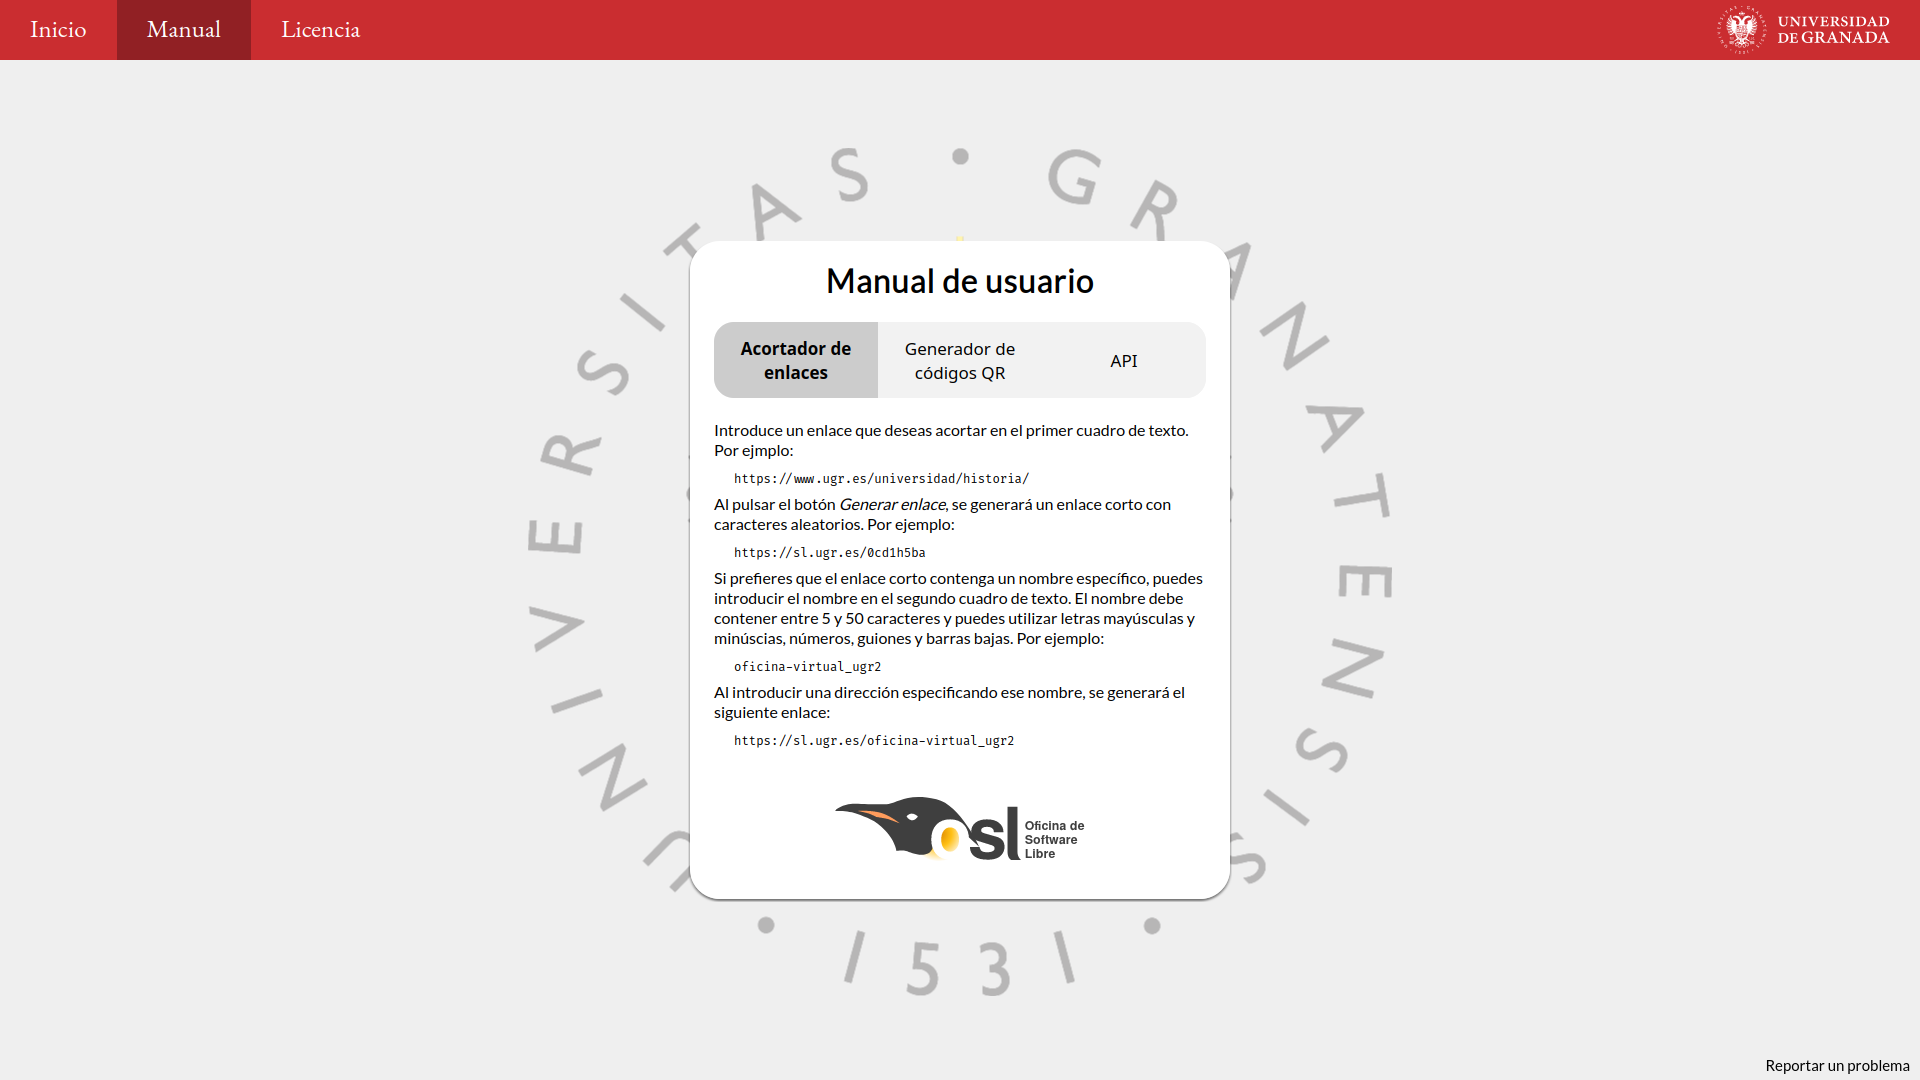
\includegraphics{web-man}
	\caption{Neosluger's manual page.}
\end{figure}

\begin{figure}[ht!]
	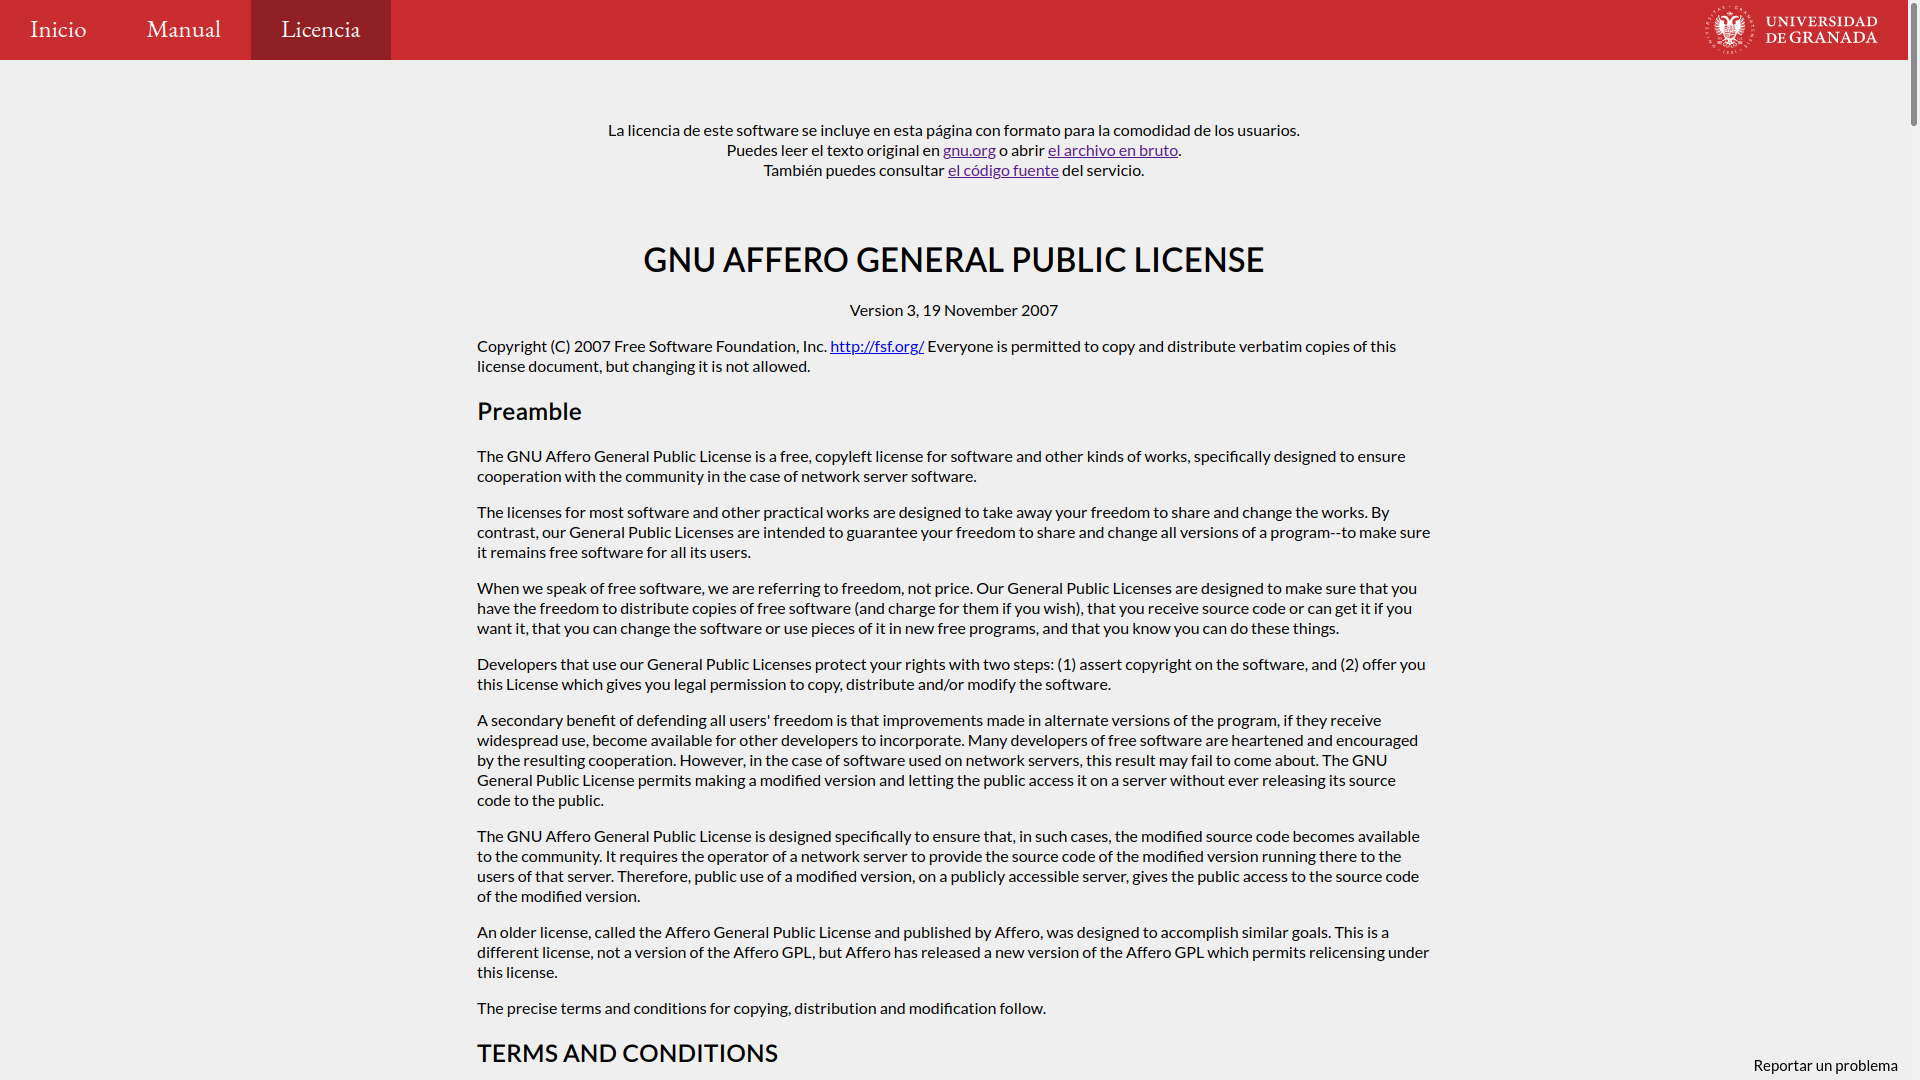
\includegraphics{web-licence}
	\caption{Neosluger's licence page.}
\end{figure}


\section{The API}\label{the-api}

Another way of accessing the service is through its API (Application Programming Interface), that allows other programs to request a short link from the service without having to use the web interface.
Its use will be further described in its own section.
\begin{figure}[ht!]
	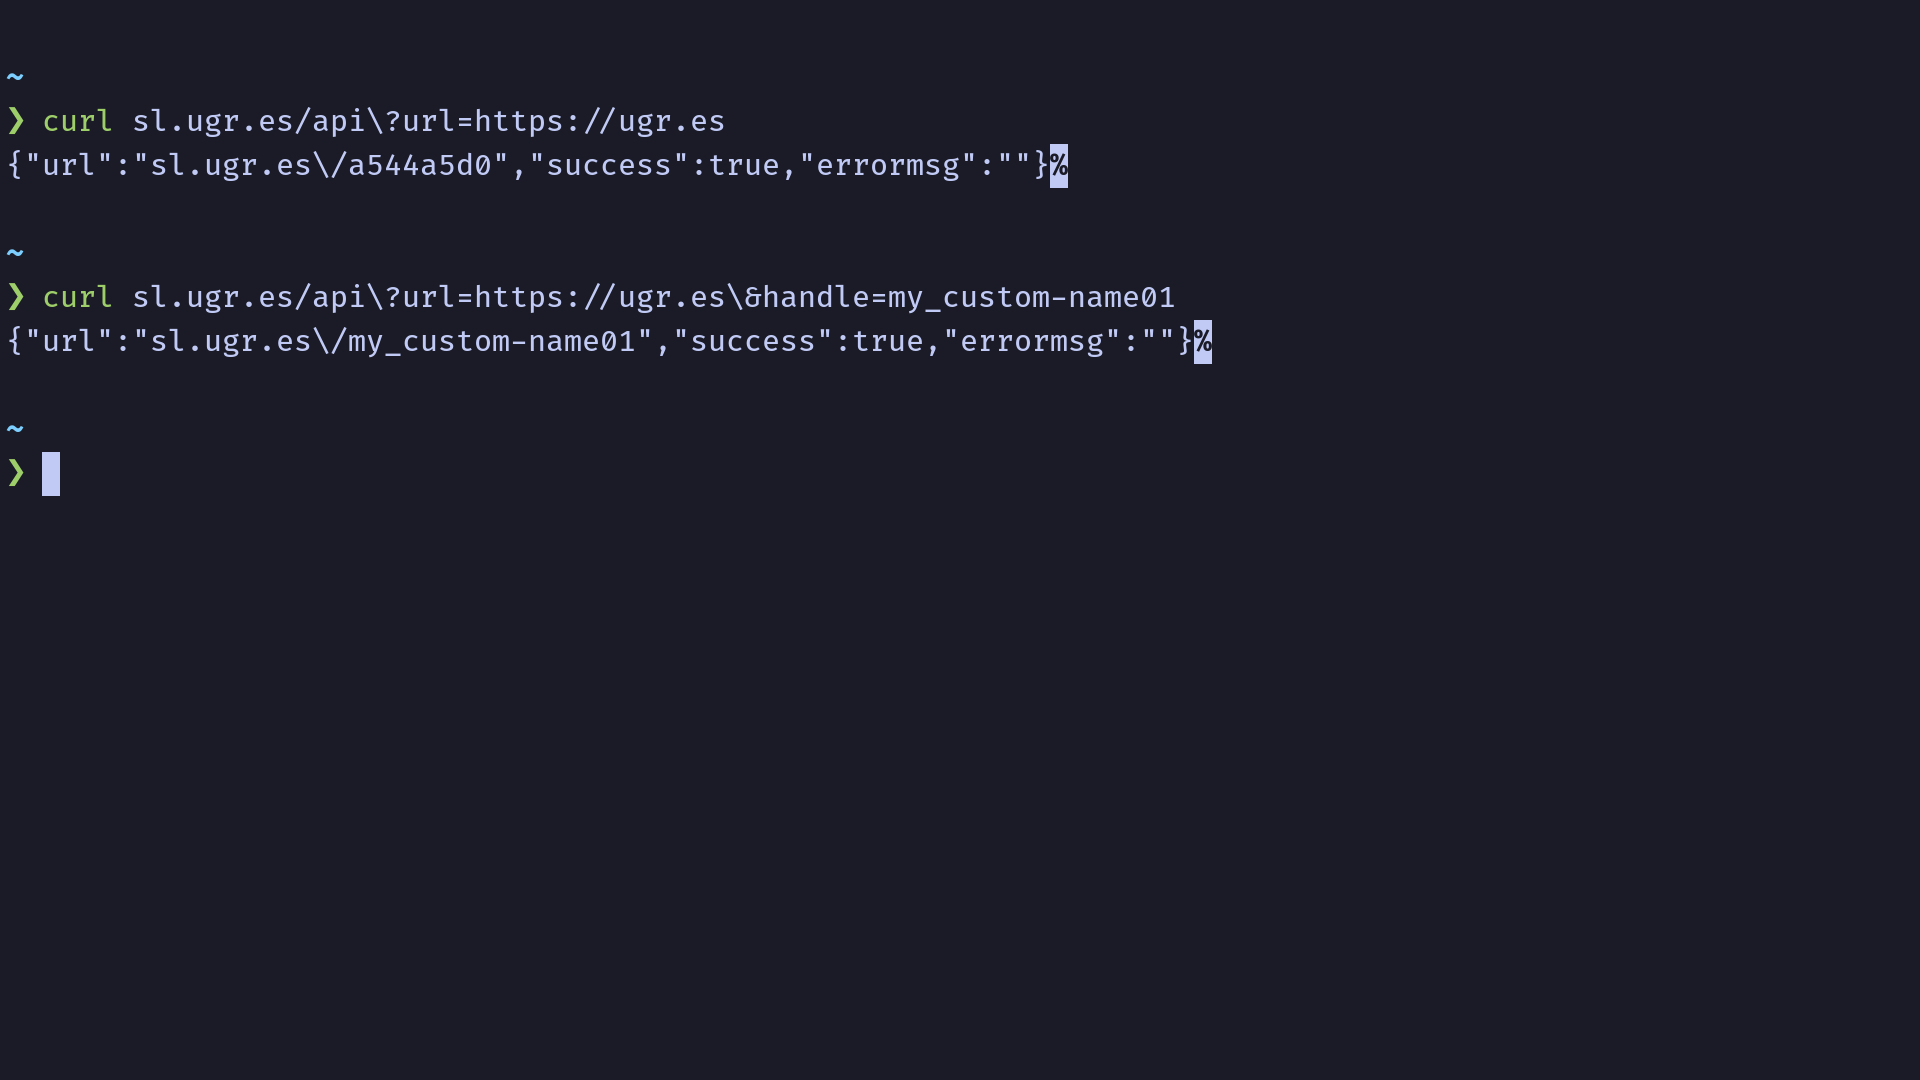
\includegraphics{api-curl}
	\caption{Short URLs creation through the API.}
\end{figure}
